\documentclass[11pt]{article}
\usepackage{hyperref} 
\usepackage{amsmath, amsfonts, amssymb}
\usepackage{graphicx}
\usepackage{float}
\usepackage[margin=1in]{geometry}

\parindent0px

\emergencystretch=0pt
\pretolerance=150
\tolerance=10000
\hbadness=10000
\hfuzz=0pt

\title{Stochastic Calculus Notes}
\author{Nathan Ueda}
\date{\today} 

\begin{document}
\maketitle 
\pagebreak
\tableofcontents 
\pagebreak

\section{Discrete Time Models}
\subsection{The One Period Model}
\subsubsection{Model Setup}
\begin{itemize}
    \item $N$ financial assets traded in this market.
    \item The assets are traded only at times $t=0$ and $t=1$.
    \item Price of asset $i$ at time $t$ is $S_i^t$.
    \item Prices of assets at time $t$ are summarized in the price vector 
    \[ \boldsymbol{s}^t = \begin{bmatrix}
        S_1^t \\
        \vdots \\ 
        S_N^t
    \end{bmatrix}\]
    \item To emphasize that $\boldsymbol{s}^1$ is not known at time $t=0$, it is random, and 
    therefore is written as $\boldsymbol{\tilde{s}}^1$.
    \item The sample space (state space) for outcomes at time $t=1$ is finite and denoted 
    $\Omega = \{\omega_1, \ldots, \omega_M\}$ 
    \item $S_1^i(\omega_j)$ denotes the price per unit of asset $i$ at time $t=1$ if $\omega_j$
    occurs. 
    \item We may therefore define the matrix $\boldsymbol{D}$ as 
    \[
    \boldsymbol{D} = 
    \begin{bmatrix}
        s^1(\omega_1) & s^1(\omega_2) & \hdots & s^1(\omega_M) 
    \end{bmatrix} =
    \begin{bmatrix}
        S_1^1(\omega_1) & S_1^1(\omega_2) & \hdots & S_1^1(\omega_M) \\
        S_2^1(\omega_1) & S_2^1(\omega_2) & \hdots & S_2^1(\omega_M) \\
        \vdots & \vdots & \ddots & \vdots \\
        S_N^1(\omega_1) & S_N^1(\omega_2) & \hdots & S_N^1(\omega_M) \\
    \end{bmatrix} \in \mathbb{R}^{N \times M}
    \]
    where column vector $i$ denotes the price of each of the $N$ assets if $\omega_i$ occurred
    and row vector $j$ denotes the price of asset $j$ in all of the $M$ possible states.
    \item We also defined the augmented matrix $\bar{\boldsymbol{D}}$ as 
    \[
    \bar{\boldsymbol{D}} = \begin{bmatrix}
        -\boldsymbol{s}^0 & \boldsymbol{D} 
    \end{bmatrix} \in \mathbb{R}^{N \times (M + 1)}
    \] 
    \item Portfolio holdings are denoted by the vector $\boldsymbol{h}$ as 
    \[
    \boldsymbol{h} = \begin{bmatrix}
        h_1 \\
        \vdots \\
        h_N
    \end{bmatrix} \in \mathbb{R}^N
    \]
    where $h_i$ denotes the number of shares held of asset $i$.
    \item The value of the portfolio at time $t=0$ is a scalar defined as 
    \[
    V^0 = \boldsymbol{h}^T \boldsymbol{s}^0 = 
    \begin{bmatrix}
        h_1 & \hdots & h_N
    \end{bmatrix} 
    \begin{bmatrix}
        S_1^1 \\
        \vdots \\ 
        S_N^1
    \end{bmatrix} \in \mathbb{R}
    \]
    \item The value of the portfolio for any of the $M$ outcomes at time $t=1$ is defined as 
    \[
    \boldsymbol{V}^1 = \boldsymbol{h}^T \boldsymbol{D} \in \mathbb{R}^{1 \times M}
    \]
    \item It follows that
    \[
    \begin{bmatrix}
        -V^0 & \boldsymbol{V}^1
    \end{bmatrix} =
    \boldsymbol{h}^T \bar{\boldsymbol{D}} \in \mathbb{R}^{1 \times (M + 1)}
    \]
\end{itemize}

\subsubsection{Assumptions}
\begin{itemize}
    \item These assumptions in the real world, but allows us to make models in a simpler 
    manner.
\end{itemize}

\textbf{Friction Free Market Assumptions}

\textbf{Behavioral Assumptions}
\begin{itemize}
    \item Agents prefer more over less. 
    \item Agents are in agreement over the states that are possible and the states that are not 
    possible. Nothing is assumed as to the probability of which each agent thinks each possible 
    outcome will occur with, as this discrepancy is how agents trade against each other.
\end{itemize}

\subsubsection{Noarbitrage}

\begin{itemize}
    \item Given the friction free and behavioral assumptions about the market, it is reasonable 
    to assume that arbitrage portfolios do not exist in the market and that it is therefore 
    \textit{arbitrage free}.
\end{itemize}

\textbf{Reachable Payoff Space}
\begin{itemize}
    \item The \textit{reachable payoff space} denotes the possible payoffs at time $t=1$ in the 
    $M$ different states. 
    \item The reachable payoff space, denoted $\mathcal{R}$, is the row space (possible linear 
    combinations of the rows) of $\boldsymbol{D}$.
    \[\mathcal{R} = \{\boldsymbol{D}^T \boldsymbol{h}: \boldsymbol{h} \in \mathbb{R}^N\} 
    \subset \mathbb{R}^M\]
    \item The augmented payoff space, denoted as $\mathcal{\bar{R}}$, is similarly defined as
    \[\mathcal{\bar{R}} = \{\boldsymbol{\bar{D}}^T \boldsymbol{h}: \boldsymbol{h} \in 
    \mathbb{R}^N\} \subset \mathbb{R}^{M+1}\]
    \item An \textit{arbitrage portfolio}, $\boldsymbol{h}$, is a portfolio for which 
    $\boldsymbol{\bar{D}}^T \boldsymbol{h} > 0$ (at least one element in the vector is strictly 
    positive). 
    \item A market is said to be \textit{arbitrage free} if there exists no arbitrage 
    portfolios. In other words, there may be many states of the world with 0 cash flows, but if
    there exists at least state with strictly positive cash flows there is arbitrage and there 
    are none where you pay anything. 
    \item Note the implications on $\bar{\boldsymbol{D}} = \begin{bmatrix} -\boldsymbol{s}^0 & 
    \boldsymbol{D} \end{bmatrix}$. If $\boldsymbol{\bar{D}}^T \boldsymbol{h} > 0$, this means we 
    had nonnegative cashflows even at time $t=0$. Put simply, this means that we don't pay 
    anything today (and maybe even earn something today) and have the possibility of positive 
    cashflows at time $t=1$ in at lesat one of the states. 
\end{itemize}

\textbf{Market Completeness}
\begin{itemize}
    \item The market is complete is $\mathcal{R}$ is all of $\mathbb{R}^M$. This can be shown 
    if Rank$(\boldsymbol{D}) = M$.
    \item If $N \ge M$, then the market may be complete (depends on the row rank).
    \item If $N < M$ the market is not complete since we can't span all of $\mathbb{R}^M$ with 
    only $N$ rows.
\end{itemize}

\textbf{State Price Vectors}
\begin{itemize}
    \item A \textit{state price vector}, denoted $\psi$, prices all the payoffs in the 
    reachable payoff space correctly and is denoted as 
    \[
    \psi = \begin{bmatrix}
        \psi_1 \\ 
        \vdots \\
        \psi_M
    \end{bmatrix} \in \mathbb{R}^{M \times 1}
    \]
    \item To get a 1 dollar payment at time $t=1$ in state $i$, $\psi_i$ is the amount needed
    to pay today at time $t=0$.
    \item Formally, it is defined as
    \[V^0 = \boldsymbol{V}^1 \psi\]
    \[\boldsymbol{s}^0 = \boldsymbol{D} \psi\]
\end{itemize}

\subsubsection{Arrow-Debreu Securities}
\begin{itemize}
    \item \textit{Arrow-Debreu securities} pay a fixed payout of 1 unit in a specified state at
    time $t=1$ and no payout in all other $M-1$ states. In other words, 

    \[ 
    \delta_i = 
    \begin{bmatrix}
        0 & 0 & \hdots & 0 & 1 & 0 & \hdots & 0 & 0
    \end{bmatrix}, \; i = 1, \ldots, M
    \]
    where $\delta_i$ pays a unit of the consumption good in state $i$ at time $t=1$.
    \item The price of $\delta_i$ at time $t=0$ is $\delta_i \psi = \psi_i$, which makes sense 
    as $\psi_i$ denotes the price of $\delta_i$ at time $t=0$.
    \item $\delta_0$ denotes a time $t=0$ Arrow-Debreu security that pays one unit at time 
    $t=0$.
\end{itemize}

\subsubsection{Fundamental Theorems of Asset Pricing}
\textbf{First Fundamental Theorem of Asset Pricing}
\begin{itemize}
    \item States that the market is arbitrage free if and only if there exists a strictly 
    positive state price vector, $\psi >> \boldsymbol{0}$.
\end{itemize}

\textbf{Second Fundamental Theorem of Asset Pricing}
\begin{itemize}
    \item Given a market that admits no arbitrage, the state price vector is unique if and only 
    if the market is complete. 
\end{itemize}

\subsubsection{Law of One Price}
\begin{itemize}
    \item This is a weaker condition than no arbitrage.
    \item LOOP is said to hold if the price today of two portfolios that make the same future
    payoff in all states must be the same. For example, if 
    \[\boldsymbol{h}_1^T \boldsymbol{D} = \boldsymbol{h}_2^T \boldsymbol{D} \implies
    \boldsymbol{h}_1^T \boldsymbol{s}^0 = \boldsymbol{h}_2^T \boldsymbol{s}^0 \]
    \item LOOP holds if and only if there exists a state price vector $\psi$.
\end{itemize}

\subsubsection{Types of Arbitrage}
\textbf{Type 1 Arbitrage}
\begin{itemize}
    \item Initial value of portfolio is nonpositive, future value is nonnegative in all 
    states, and strictly positive in at least one state. 
    \item This means that at time $t=0$, we pay nothing to take it, and we have the possibility 
    of generating strictly positive cash flows at time $t=1$.
    \item Put simply, type 1 arbitrage generates strictly positive cash flows in the future in 
    some state. 
\end{itemize}

\textbf{Type 2 Arbitrage}
\begin{itemize}
    \item Initial value of portfolio is negative (you get paid to take it) and future value of 
    portfolio is nonnegative in all states.
    \item This means that at time $t=0$, we have a strictly positive cash flow, and we will 
    never have negative cash flows at time $t=1$.
    \item Put simply, type 2 arbitrage generates strictly positive cash flows immediately.
\end{itemize}

\textbf{Type 1 and 2 Arbitrage}
\begin{itemize}
    \item Initial value of portfolio is negative (type 2) and future value is strictly positive 
    in at least one state.
    \item This means that at time $t=0$, we are paid to take the portfolio and at time $t=1$ 
    we have a strictly positive probability of generating a positive cash flow.
\end{itemize}

\subsubsection{Risk Neutral Probabilities}
\begin{itemize}
    \item Artifical probabilities (not true probabilities) that are useful from a pricing 
    perspective but have no real world intepretations as probabilities.
    \item The reason we call these probabilities is that they behave like probabilities (they
    satisfy the Kolmogorov axioms of probability).
    \item They summarize the information in the state price vector.
\end{itemize}

\textbf{Setup}
\begin{itemize}
    \item A r.v. is a function $\tilde{X}: \Omega \rightarrow \mathbb{R}$. In other words, it 
    is a function from the sample space to a real number. 
    \item For now, we focus on discrete sample spaces.
    \item The expectation of a r.v. is 
    \[E_{\mathbb{P}}[\tilde{X}] = \sum_{i} \tilde{X}(\omega_i)\mathbb{P}(\omega_i)\]
    \item It is possible to have two probability measures $\mathbb{P}$ and $\mathbb{Q}$ defined 
    over the same sample space. 
    \begin{itemize}
        \item If $\mathbb{P}$ and $\mathbb{Q}$ are in agreement over which events have a 
        probability of 0, then they are equivalent. 
        \[\mathbb{P}(A) = 0 \iff \mathbb{Q}(A) = 0\]
        \item $\mathbb{Q}$ is absolutely continuous w.r.t. $\mathbb{P}$, denoted $\mathbb{Q} << 
        \mathbb{P}$, if $\mathbb{P}(A) = 0 \implies \mathbb{Q}(A) = 0$.
        \item If $\mathbb{Q} << \mathbb{P}$, we can define the \textit{Radon-Nikodym} 
        derivative (likelihood ratio) of $\mathbb{Q}$ w.r.t. $\mathbb{P}$ (how much 
        $\mathbb{Q}$ probability is assigned to an event w.r.t to how much $\mathbb{P}$ 
        probability is assigned to an event)
        \[L(A) = \frac{d\mathbb{Q}}{d\mathbb{P}} = \frac{\mathbb{Q}(A)}{\mathbb{P}(A)}, \; 
        \mathbb{P}(A) > 0\]
        from this is follows that, for any r.v. $\tilde{X}$
        \[E_{\mathbb{P}}[L\tilde{X}] = E_{\mathbb{Q}}[\tilde{X}]\]
    \end{itemize}
\end{itemize}

\textbf{Risk Neutral Setup}
\begin{itemize}
    \item We can now do some redefining of the model using these risk neutral probabilities
    \item For portfolio $\boldsymbol{h} \in \mathbb{R}^N$, the payoff in the form of a r.v. at 
    time $t=1$ if $\omega_i$ occurred is defined 
    \[\tilde{V}^1(\omega_i) = {(\boldsymbol{h}^T \boldsymbol{D})}_i\]
    Instead of having a vector $\boldsymbol{V}^1$, we now $\tilde{V}^1$ r.v.
    \item We assume the vector of ones, $\boldsymbol{1}$ is in the payoff space, that is, 
    $\boldsymbol{1} \in \mathcal{R}$. This implies that there is a risk free asset, or some 
    portfolio that generates exactly the payoffs of the risk free asset, and the price of that
    portfolio can determine the unique risk free rate (unique since we assume there is no 
    arbitrage, if it there were multiple risk free rates, there would be arbitrage), defined 
    \[R = 1 + r = \frac{1}{\hat{\psi}}\] 
    where 
    \[\hat{\psi} = \sum_{i=1}^{M} \psi_i = \boldsymbol{1} \psi\]
    for state price vector $\psi$.
    \item We can now define the \textit{risk-neutral probabilities}, $q_1, \ldots, q_M$, where 
    \[q_i = \frac{\psi_i}{\psi}\]
    and these $q$'s make up the corresponding equivalent probability measure $\mathbb{Q}$.
    \item The higher the value $q_i$ is, the more we are willing to pay for that state. 
    \item In the form of a discounted expectation, it now follows that
    \[V^0 = \frac{1}{R}E_{\mathbb{Q}}[\tilde{V}^1]\]
    for all payoffs in $\mathcal{R}$. This is just a reinterpreation, but a very important one 
    as it allows us to use fancy stochastic methods for thinking about asset pricing. 
    \item Similarly, it follows that 
    \[V^0 = \frac{1}{R}E_{\mathbb{P}}[L\tilde{V}^1]\]
\end{itemize}

\textbf{Risk Neutral Probabilities}
\begin{itemize}
    \item The measure $\mathbb{Q}$ is called the \textit{risk-neutral measure}.
    \item A one period random process, $X_t, \; t=0,1$ is called a \textit{martingale} (or 
    $\mathbb{Q}$-martingale) if its value at time $t=0$ is equal to its expected value at time 
    $t=1$, that is
    \[E_{\mathbb{Q}}[X_1] = X_0\]
    In other words, the best estimate of the value tomorrow is the value today.
    \item Defining the random process $M$, by $M_0=1$ and $M_1=\frac{1}{R}L$, it then follows 
    that 
    \[M_0 V^0 = E_{\mathbb{P}}[M_1 V^1]\]
    which also shows that $MV$ is a $\mathbb{P}$-martingale.
    \item $M$ is called suitably called the \textit{stochastic discount factor}, as it is a 
    discount factor (the price today as a function of the price tomorrow) and it is stochastic.
    \item As long as there is noarbitrage, there is always a stochastic discount factor. 
    \item Given the discounted process $\hat{V}_0 = V_0$ and $\hat{V}^1 = \frac{\tilde{V}}{R}$,
    we have 
    \[\hat{V}_0 = E_{\mathbb{Q}}[\hat{V}_1]\]
    therefore $\mathbb{Q}$ is called the \textit{equivalent martingale measure}.
\end{itemize}

\subsubsection{Risk Neutral Fundamental Theorems}
\begin{itemize}
    \item We can reformulate the fundamental theorems as a statement about risk neutral
    measures and equivalent martingale measures.
\end{itemize}

\textbf{Risk Neutral First Fundamental Theorem}
\begin{itemize}
    \item The market is arbitrage free if and only if there exists an equivalent martingale 
    maeasure, $\mathbb{Q}$, such that the price of any asset in $\mathcal{R}$ is given by 
    $V^0 = \frac{1}{R}E_{\mathbb{Q}}[\tilde{V}^1]$
\end{itemize}

\textbf{Risk Neutral Second Fundamental Theorem}
\begin{itemize}
    \item Given a market that admits no arbitrage, the equivalent martingale measure is unique 
    if and only if the market is complete.
\end{itemize}

\subsubsection{Summary}

\begin{itemize}
    \item $V_0$ may be written in many equivalent manners 
    \begin{itemize}
        \item Using the state price vector 
        \[V_0 = \boldsymbol{V}^1 \psi\]
        \item Using equivalent martingale measure/risk neutral probabilities 
        \[V_0 = \frac{1}{R} E_{\mathbb{Q}}[\tilde{V}^1]\]
        where $q_i = \frac{\psi_i}{\hat{\psi}}, R = \frac{1}{\hat{\psi}}$.
        \item Using the likelihood ratio 
        \[V_0 = \frac{1}{R} E_{\mathbb{P}}[L\tilde{V}^1]\]
        where $L_i = \frac{q_i}{p_i}$.
    \end{itemize}
    
\end{itemize}

\subsection{The Binomial Model}

\subsubsection{Notation}
\begin{itemize}
    \item $S$: value of the underlying asset.
    \item $C$: value of the call option.
    \item $P$: value of the put option.
    \item $K$: exercise price of the option.
    \item $r$: one period net risk free interest rate.
    \item $R$: one period gross risk free interest rate ($1+r$).
\end{itemize}

\subsubsection{Options}

\begin{figure}[H] 
    \centering 
    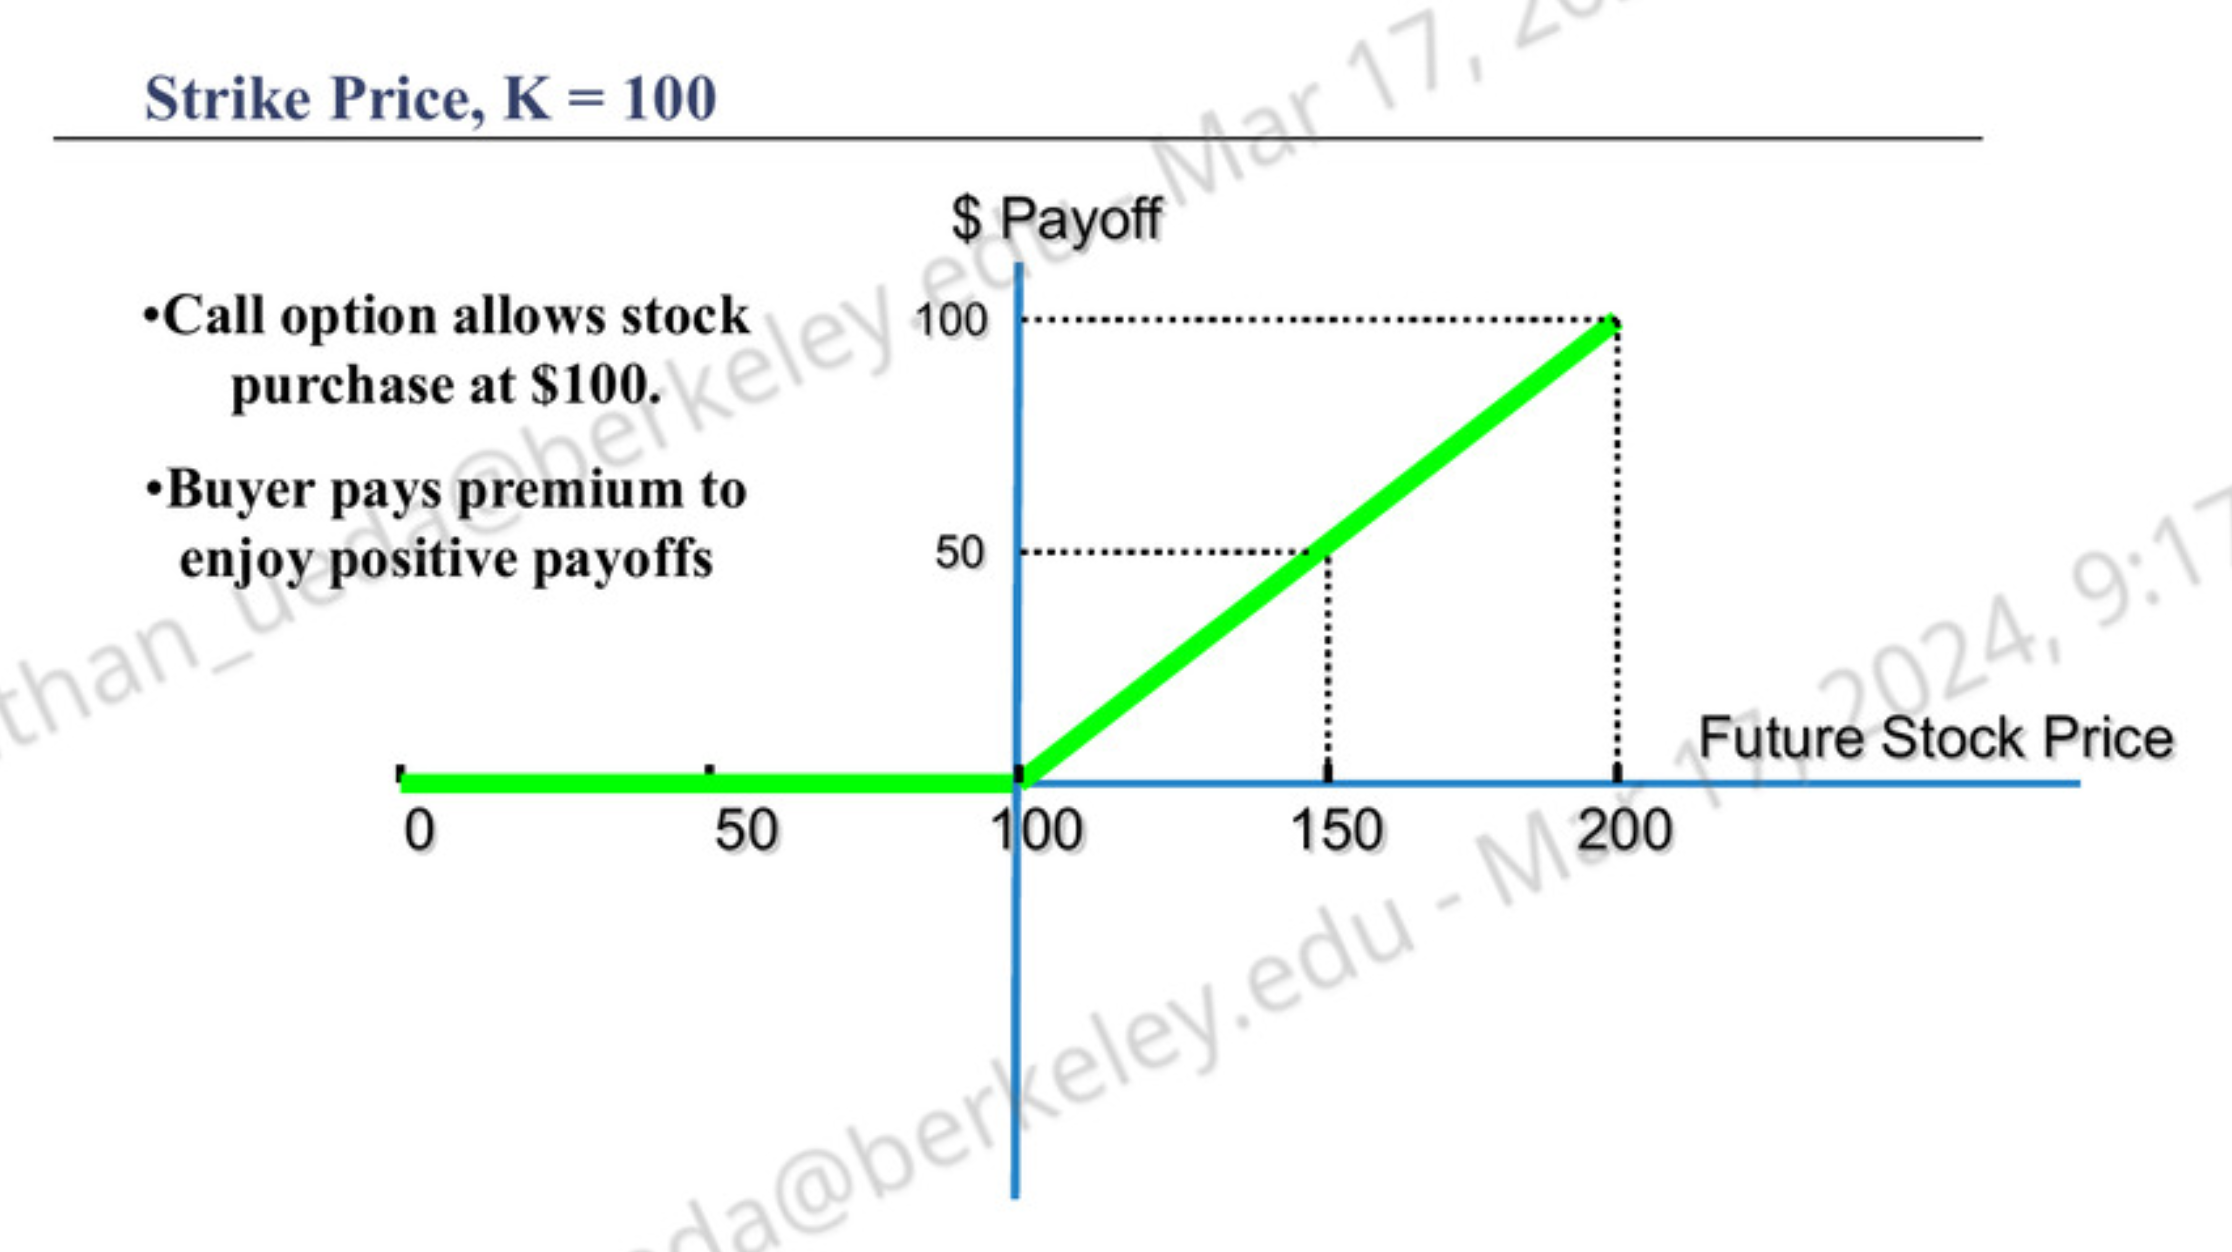
\includegraphics[width=4in]{imgs/call_payoff.png}
    \caption{Call payoff at expiration.}
\end{figure}

\begin{figure}[H] 
    \centering 
    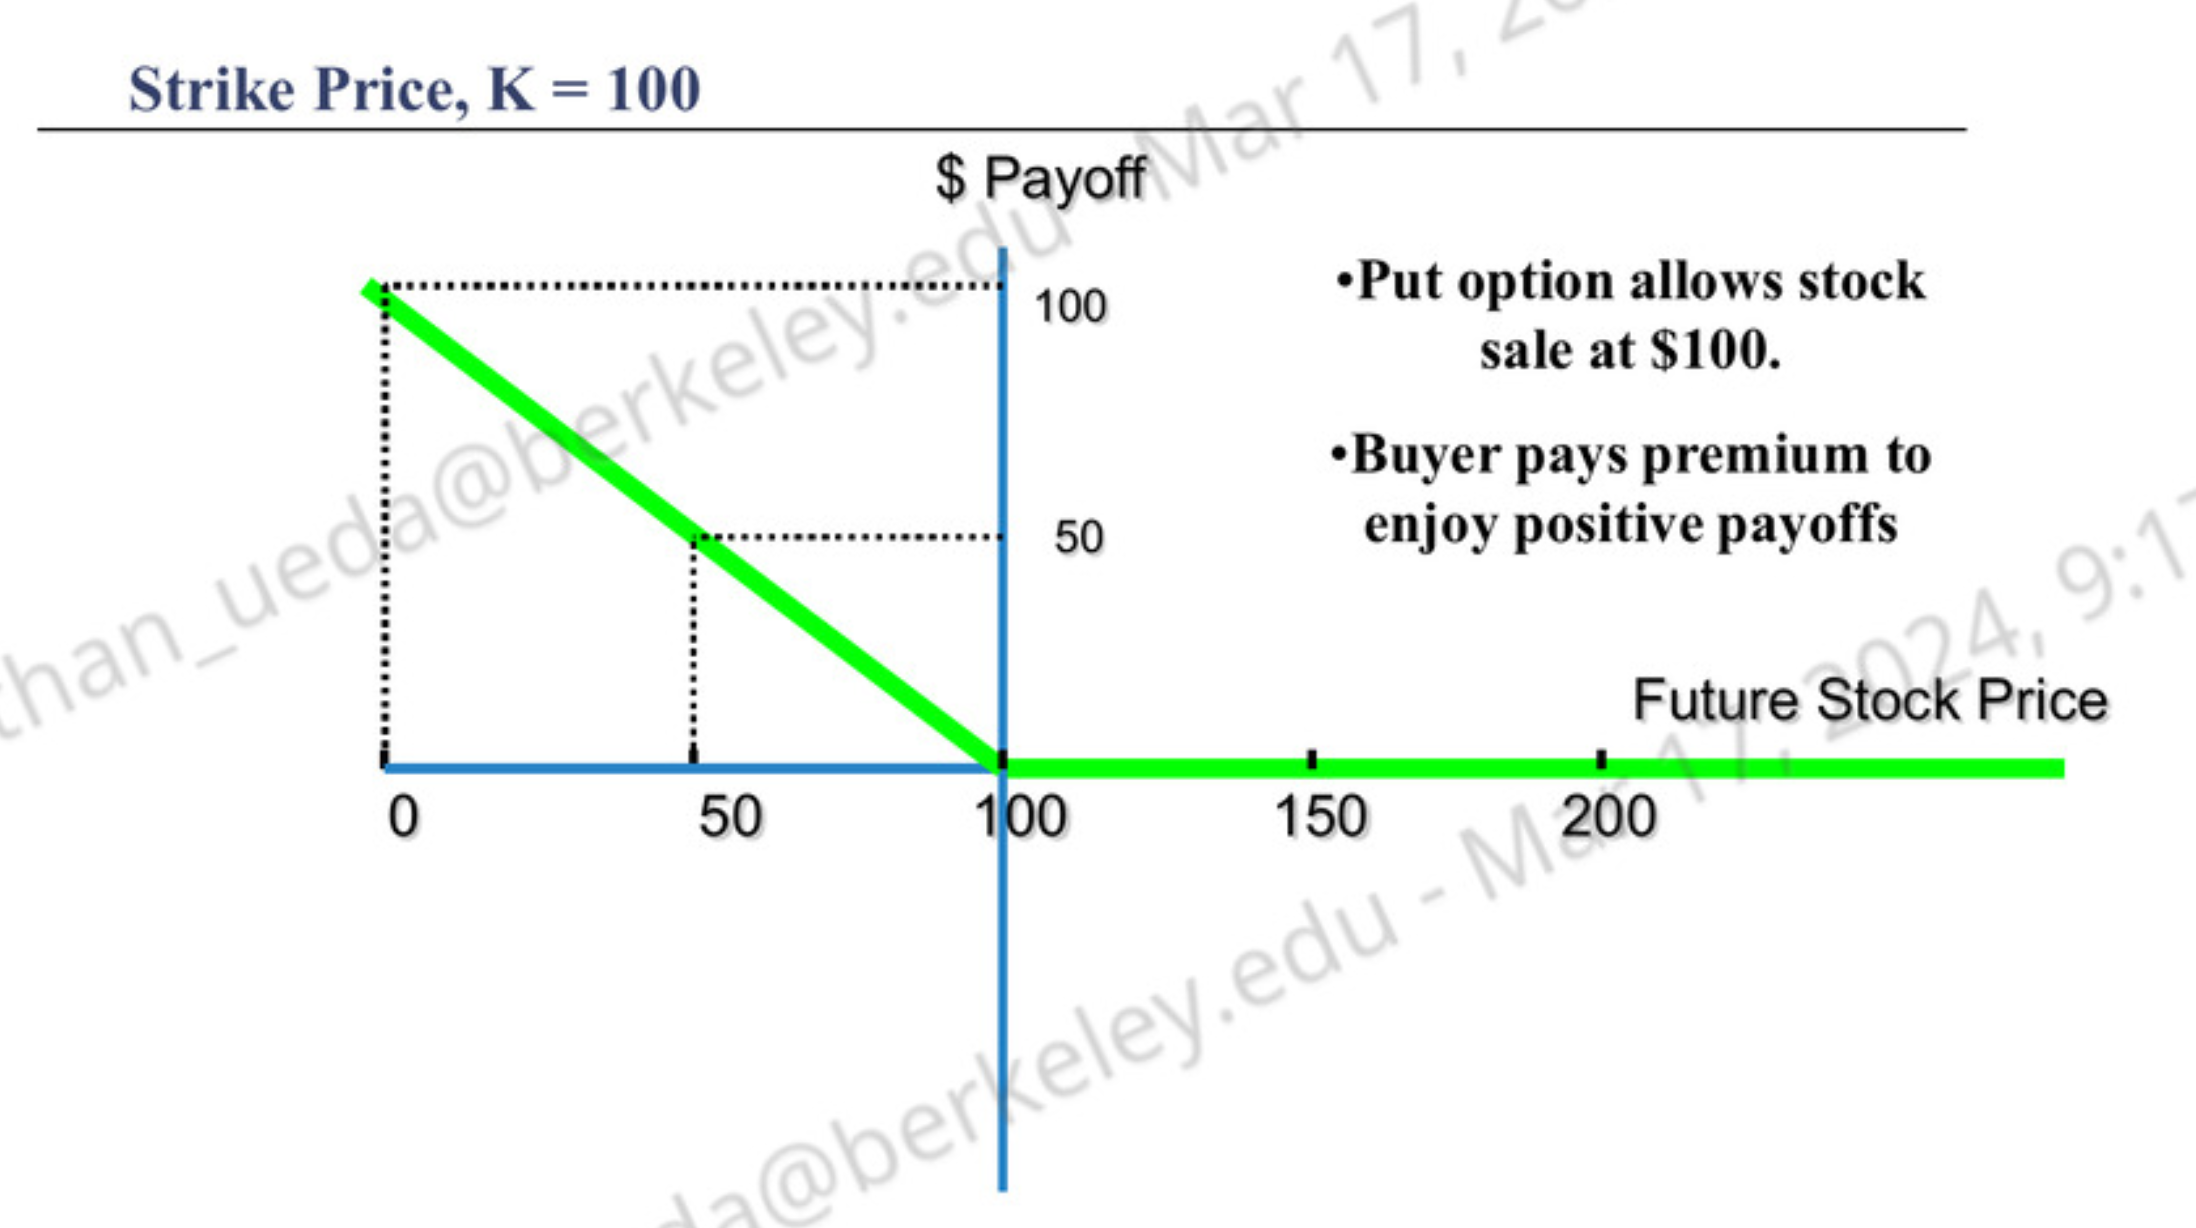
\includegraphics[width=4in]{imgs/put_payoff.png}
    \caption{Put payoff at expiration.}
\end{figure}

\textbf{Formulas for Options Payoffs}
\begin{itemize}
    \item Call: $C = \text{Max}[0, S-K]$
    \item Put: $P = \text{Max}[0, K-S]$
\end{itemize}

\subsubsection{One Period, Two State Binomial Model}
\begin{itemize}
    \item Two points in time: $t=0$ and $t=1$
    \item Two assets: a bond and a stock 
    \item Price of bond at time $t$ is denoted $B_t$
    \item Price of stock at time $t$ is denoted $S_t$
    \item The bond price is deterministic and given by 
    \[B_0 = 1\]
    \[B_1 = R\]
    where $R \ge 1$.
    \item The stock price is a stochastic process where 
    \[S_0 = S\]
    \[
    S_1 = \begin{cases}
        uS, & \text{with probability } p_u \\
        dS, & \text{with probability } p_d
    \end{cases}
    \] where $u \ge d$.

    \begin{figure}[H] 
        \centering 
        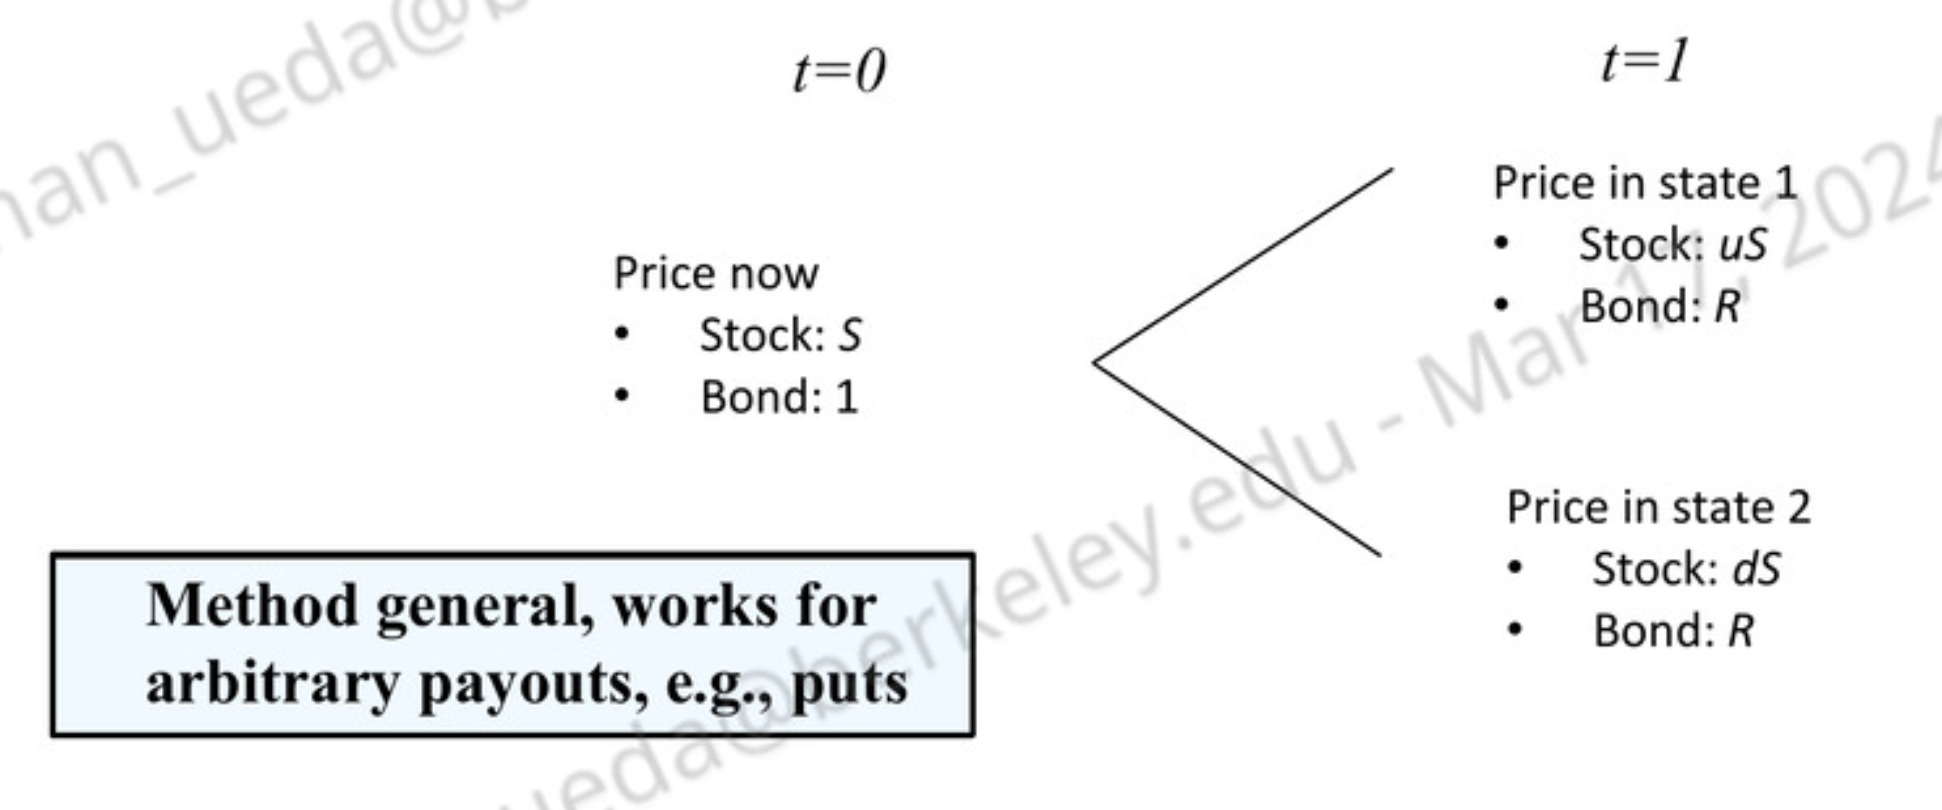
\includegraphics[width=4in]{imgs/one_period_two_state_bin_tree_model.png}
        \caption{Price dynamics}
    \end{figure}
    \item Within our framework, this can be setup as 
    \[
    \boldsymbol{s}_0 = \begin{bmatrix}
        1 \\ 
        1
    \end{bmatrix}
    \]
    \[ 
    \boldsymbol{D} = \begin{bmatrix}
        u & d \\
        R & R \\
    \end{bmatrix}
    \]

    \item Payoff for call will be either 
    \[C_u = \text{max}(uS - K, 0)\]
    or 
    \[C_d = \text{max}(dS - K, 0)\]
\end{itemize}





\section{Appendix}
\subsection{Operator Overloading}
For some vector $\boldsymbol{a}$, we write
\begin{itemize}
    \item $\boldsymbol{a} \ge \boldsymbol{0}$ if all elements are nonnegative
    \item $\boldsymbol{a} > \boldsymbol{0}$ if at least one element is strictly positive
    \item $\boldsymbol{a} >> \boldsymbol{0}$ if all elements are strictly positive
\end{itemize}
Similarly,
\begin{itemize}
    \item $\boldsymbol{a} \le \boldsymbol{0}$ if all elements are nonpositive
    \item $\boldsymbol{a} < \boldsymbol{0}$ if at least one element is strictly negative
    \item $\boldsymbol{a} << \boldsymbol{0}$ if all elements are strictly negative
\end{itemize}
\end{document}
